\chapter{Colposcopy}

\section*{Overview}
Colposcopy is a close examination of the cervix, and sometimes the vagina or vulva, using a magnifying instrument called a colposcope. The instrument stays outside the body; a speculum is used to see the cervix. Colposcopy is commonly recommended after certain abnormal cervical screening results or when the cervix looks unusual. A small biopsy may be taken, but not every examination includes one.


\begin{center}
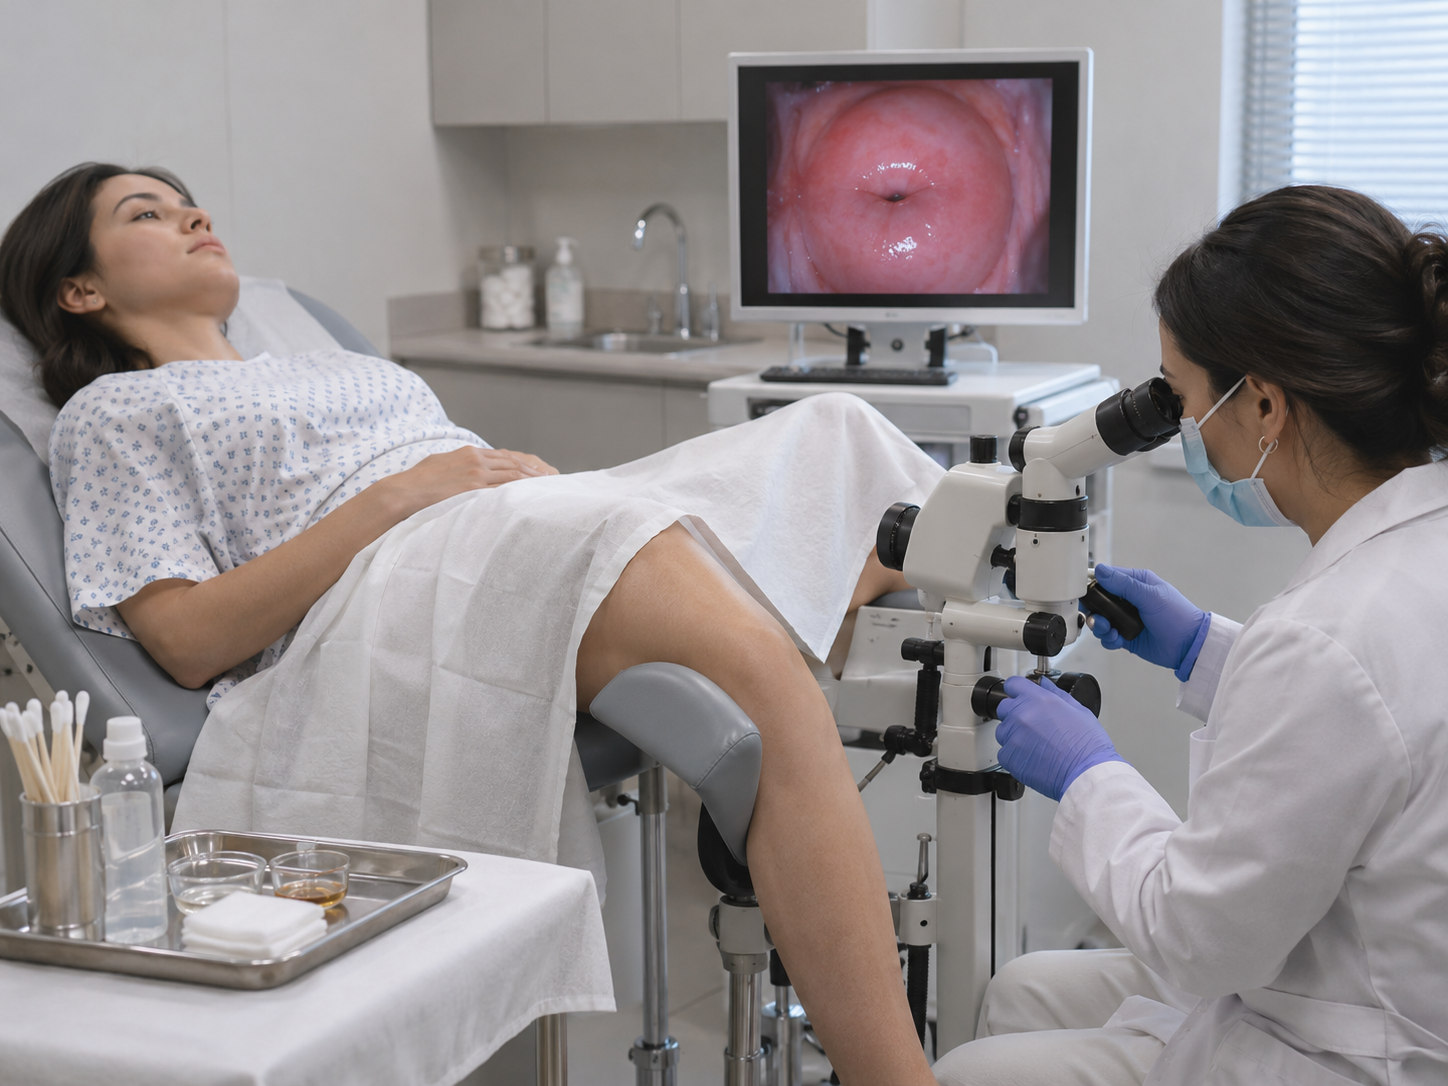
\includegraphics[width=0.82\textwidth]{images/chapters/procedure_colposcopy_overview.png}
\captionof{figure}{Conceptual overview of Colposcopy. Not a procedural guide.}
\end{center}
\section*{Alternative Names}
Colposcopic examination; colposcopy with cervical biopsy (when tissue is sampled).

\section*{Principle}
The clinician looks at the cervix under magnification and may apply a weak vinegar-like solution (acetic acid), and sometimes an iodine solution, to help distinguish areas that may need closer assessment. If indicated, small tissue samples are taken from suspicious areas and examined in a laboratory. Colposcopy provides an appearance-based assessment; biopsy results, when taken, provide the tissue diagnosis.

\section*{History}
Hans Hinselmann developed the colposcope in the 1920s as a way to examine the cervix more closely. Colposcopy later became an important follow-up procedure for abnormal cervical screening results.

\section*{Why It Is Done}
Colposcopy may be recommended after an abnormal Pap test, a positive high-risk HPV test, repeated abnormal screening results, or a visible cervical change or symptom that needs evaluation. Whether it is needed depends on the exact result, prior screening history, age, and other risk factors; not every abnormal screening result requires immediate colposcopy.

\section*{Role in Care}
Colposcopy is usually a diagnostic follow-up examination, not a screening test. It may be performed with a biopsy or followed by another procedure depending on what is seen and on the person's prior results.

\section*{How It Is Performed}
The patient lies on an exam table, and a speculum gently opens the vagina so the cervix can be seen. The clinician examines the cervix with the colposcope and may apply solutions to highlight areas. If a biopsy is needed, a small piece of tissue is pinched from the cervix; this can cause a brief pinch or cramp. A sample from inside the cervical canal may sometimes be collected in nonpregnant patients. The visit commonly takes 10 to 20 minutes, though it can take longer.

\section*{Preparation}
Follow the clinic's instructions. Tell the clinician if you may be pregnant, have an allergy to latex or a solution that may be used, take blood-thinning medicine, or have a bleeding disorder. Do not stop prescribed medicine unless your clinician tells you to. Some clinics advise avoiding vaginal sex, tampons, or vaginal medicines for a short time beforehand; practices vary. If you have heavy menstrual bleeding on the appointment day, call the clinic to ask whether the examination should be rescheduled. You may ask to pause the exam at any time or request a support person or chaperone according to local practice.

\section*{Contraindications and Precautions}
Colposcopy itself usually has no absolute contraindication, but active heavy bleeding or severe discomfort may limit the examination. Pregnancy does not automatically prevent colposcopy or a directed biopsy when needed. Because the cervix is more vascular during pregnancy, the clinician should be experienced; endocervical curettage is not performed during pregnancy, and treatment of precancer is generally deferred until after pregnancy unless cancer is suspected. The plan is based on the person's screening risk and clinical findings.

\section*{Risks}
Without a biopsy, colposcopy usually causes little or no lasting discomfort. A biopsy can cause brief cramping and light bleeding or discharge for several days. Infection or heavier bleeding is uncommon. If treatment such as LEEP or cone biopsy is recommended later, it is a separate procedure with additional risks that should be discussed separately.

\section*{Aftercare and Recovery}
Most people return to usual activities the same day. If a biopsy was taken, light spotting or dark discharge can occur, especially if a medicine was applied to stop bleeding. Follow the clinic's instructions about pads, tampons, vaginal sex, and activity; restrictions are usually needed only while bleeding or discharge continues and may vary by clinic. Biopsy results often take a few weeks, but timing varies.

\section*{Outcome and Follow-up}
The clinician may describe the appearance during the visit. If a biopsy was taken, the laboratory may report normal tissue or cervical intraepithelial neoplasia (CIN) grade 1, 2, or 3. CIN is a description of abnormal cells and is not the same as invasive cancer. Follow-up depends on the biopsy, HPV and screening results, prior history, age, and pregnancy status. Options may include repeat HPV-based testing or cytology, repeat colposcopy, or treatment of higher-grade precancer. Some low-grade changes resolve without treatment. During pregnancy, high-grade changes may need monitoring during pregnancy or reassessment after delivery; treatment is usually delayed until after birth unless cancer is suspected. When postpartum colposcopy is recommended, ASCCP advises scheduling it no sooner than 4 weeks after delivery. The clinician will explain the result and specific follow-up plan.

\section*{When to Seek Medical Care}
Contact the clinic promptly for bleeding heavier than a normal period, bleeding that does not ease, fever or chills, foul-smelling discharge, or worsening pelvic pain. Seek urgent care for severe pain, heavy bleeding with dizziness or fainting, or if you feel seriously unwell. Follow the clinic's instructions for aftercare and whom to contact.

\section*{References}
\begin{enumerate}
  \item National Health Service (NHS). Colposcopy. https://www.nhs.uk/tests-and-treatments/colposcopy/ (accessed November 23, 2026).
  \item American Society for Colposcopy and Cervical Pathology (ASCCP). 2019 Risk-Based Management Consensus Guidelines for Abnormal Cervical Cancer Screening Tests and Cancer Precursors, with updates. https://www.asccp.org/guidelines (accessed November 23, 2026).
  \item ASCCP. Management of Abnormal Cervical Cancer Screening Tests in Pregnancy. Practice Pearl. https://www.asccp.org/practice-pearls (accessed November 23, 2026).
  \item ASCCP. Colposcopy Standards: Guidelines for Endocervical Curettage at Colposcopy. \textit{Journal of Lower Genital Tract Disease}. 2023;27(1):97--101. https://doi.org/10.1097/LGT.0000000000000710 (accessed November 23, 2026).
  \item National Cancer Institute (NCI). Enduring Consensus Cervical Cancer Screening and Management Guidelines. https://dceg.cancer.gov/research/cancer-types/cervix/enduring-guidelines (accessed November 23, 2026).
\end{enumerate}
\clearpage
